% SC4012 --- Chapter 5: Fuzzing, Sanitizers and Symbolic Execution (0->100 ground-up)
\chapter{Fuzzing, Sanitizers and Symbolic Execution}
\label{ch:fuzzing}

\begin{quote}
\emph{``If you have not fuzzed it, it is not tested.''} --- Fuzzing, sanitizers and symbolic reasoning turn ``does it work on my input'' into ``does it survive an adversary who controls the input.''
\end{quote}

\noindent\fbox{\parbox{\dimexpr\linewidth-2\fboxsep-2\fboxrule}{%
\textbf{From zero: why testing misses bugs.} We start from random testing, add coverage guidance, then add oracles that notice memory errors, then add solving to reach deep branches. No prior testing background assumed.}}
\vspace{0.4em}

\section*{Learning Outcomes}
After this chapter you will be able to:
\begin{enumerate}[label=(L\arabic*)]
    \item explain coverage-guided fuzzing and why it beats black-box random;
    \item run AFL++/libFuzzer and interpret corpus, coverage and crashes;
    \item describe ASan/UBSan/MSan and what each detects at runtime;
    \item contrast fuzzing, symbolic execution and concolic execution (trade-offs);
    \item triage a crash (deduplicate, minimise, root-cause and patch).
\end{enumerate}

% ============================================================
\section{Coverage-Guided Fuzzing}
\label{sec:fuzzing}
Intuition: a fuzzer is a very fast, very dumb adversary that tries millions of mutated inputs and keeps those that discover new code. A \emph{coverage-guided} fuzzer instruments the program so each input reports which branches it hit; inputs that cover new edges are added to the corpus and mutated further.

\begin{definition}[Fuzzing loop]
Seed corpus $C$; queue $Q=C$. Loop: pick $t\in Q$, mutate to $t'$, execute $P(t')$, collect coverage $Cov(t')$ and crash signal. If $Cov(t')\not\subseteq \bigcup Cov(Q)$, add $t'$ to $Q$. If $P$ crashes (ASan, assert, timeout), save $t'$ as bug. Cycle until budget expires.
\end{definition}

\begin{figure}[h]\centering
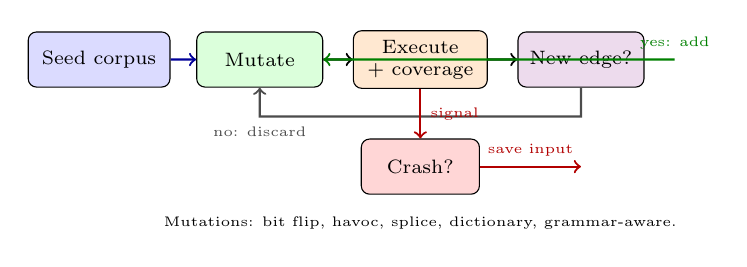
\begin{tikzpicture}[scale=0.85,every node/.style={font=\scriptsize}]
  \node[draw,fill=blue!14,rounded corners=3pt,minimum width=1.8cm,minimum height=0.7cm,align=center] (seed) at (-4.2,1.6) {Seed corpus};
  \node[draw,fill=green!14,rounded corners=3pt,minimum width=1.6cm,minimum height=0.7cm,align=center] (mut) at (-1.8,1.6) {Mutate};
  \node[draw,fill=orange!18,rounded corners=3pt,minimum width=1.7cm,minimum height=0.7cm,align=center] (exec) at (0.6,1.6) {Execute\\+ coverage};
  \node[draw,fill=violet!14,rounded corners=3pt,minimum width=1.6cm,minimum height=0.7cm,align=center] (cov) at (3.0,1.6) {New edge?};
  \node[draw,fill=red!16,rounded corners=3pt,minimum width=1.5cm,minimum height=0.7cm,align=center] (crash) at (0.6,0) {Crash?};
  \draw[->,thick,blue!60!black] (seed) -- (mut);
  \draw[->,thick] (mut) -- (exec);
  \draw[->,thick] (exec) -- (cov);
  \draw[->,thick,green!50!black] (cov) -- ++(1.4,0) |- (mut) node[near start,above,font=\tiny] {yes: add};
  \draw[->,thick,gray!60!black] (cov) -- ++(0,-0.85) -| (mut) node[midway,below,font=\tiny] {no: discard};
  \draw[->,thick,red!70!black] (exec) -- (crash) node[midway,right,font=\tiny] {signal};
  \draw[->,thick,red!70!black] (crash) -- ++(2.4,0) node[midway,above,font=\tiny] {save input};
  \node[font=\tiny,align=center] at (0.6,-0.85) {Mutations: bit flip, havoc, splice, dictionary, grammar-aware.};
\end{tikzpicture}
\caption{Coverage-guided fuzzing loop. Coverage feedback retains only inputs that expand the frontier; sanitizers turn silent corruption into a crash so the fuzzer notices it.}
\label{fig:fuzz-loop}
\end{figure}

Black-box random finds shallow bugs; coverage guidance finds deep ones because each new edge is a stepping stone. Dictionaries (known tokens like \texttt{<script>}, \texttt{--}, PNG magic) and grammars (for parsers, JS engines, SQL) help cross syntactic checks that random bytes cannot. Coverage-guided fuzzing amplified by dictionaries discovered Heartbleed-class bugs where a length field was trusted without validation.

 like \texttt{<script>}, \texttt{--}) and grammars (for parsers) help cross syntactic checks that random bytes cannot.

\begin{lstlisting}[language=C]
// libFuzzer harness: the fuzzer calls this with arbitrary bytes
#include <stdint.h>
#include <stddef.h>
int LLVMFuzzerTestOneInput(const uint8_t *data, size_t size) {
    // target API under test; crashes/sanitizer reports are bugs
    parse_header(data, size);
    return 0;
}
// Build: clang -fsanitize=address,fuzzer -g harness.c parser.c -o fuzzer
// Run: ./fuzzer corpus/ -max_total_time=60
\end{lstlisting}

Throughput is king: a good fuzzer executes $10^4$--$10^6$ inputs/sec. Keep the harness small, avoid file I/O, seed with valid samples, and reset global state per iteration. Use \texttt{afl-cmin} to minimise the corpus and \texttt{AFL\_DICTIONARY} for format-aware tokens. Structured fuzzers (libprotobuf-mutator, Nautilus) generate syntactically valid inputs for parsers, reaching deeper than raw byte flips.

 a good fuzzer executes $10^4$--$10^6$ inputs/sec. Keep the harness small, avoid file I/O, seed with valid samples, and reset global state per iteration.

\begin{lstlisting}[language=Python]
# Python fuzzing with Atheris (libFuzzer for Python)
import atheris, sys
import my_parser
def TestOneInput(data):
    try: my_parser.parse(data)
    except my_parser.ParseError: pass  # expected; not a bug
atheris.Setup(sys.argv, TestOneInput)
atheris.Fuzz()
\end{lstlisting}

% ============================================================
\section{Sanitizers: Turning Silent Corruption into Crashes}
\label{sec:sanitizers}
Most memory bugs are silent: an overflow corrupts but does not crash until later, so a fuzzer would miss it. Sanitizers instrument the build to detect errors at the moment they occur and abort with a report.

\begin{description}[leftmargin=1.2em,itemsep=0.35em]
    \item[AddressSanitizer (ASan)] Shadow memory tracks which bytes are addressable; every load/store is checked. Detects overflow, UAF, double-free, with $\sim2\times$ slowdown and $\sim2\times$ memory.
    \item[UndefinedBehaviorSanitizer (UBSan)] Checks signed overflow, shift past width, misaligned/null deref.
    \item[MemorySanitizer (MSan)] Tracks uninitialised reads; needs full rebuild and is invaluable for info-leak bugs where an uninitialised buffer is sent to the network (Heartbleed was an over-read of uninitialised-adjacent memory; MSan would have flagged the source, ASan the over-read).
    \item[ThreadSanitizer (TSan)] Detects data races; complementary to ASan.
\end{description}

\begin{figure}[h]\centering
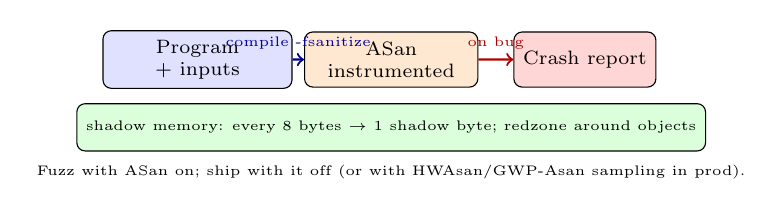
\begin{tikzpicture}[scale=0.82,every node/.style={font=\scriptsize}]
  \node[draw,fill=blue!12,rounded corners=3pt,minimum width=2.4cm,minimum height=0.7cm,align=center] (prog) at (-3.0,1.2) {Program\\+ inputs};
  \node[draw,fill=orange!18,rounded corners=3pt,minimum width=2.2cm,minimum height=0.7cm,align=center] (asan) at (0,1.2) {ASan\\instrumented};
  \node[draw,fill=red!16,rounded corners=3pt,minimum width=1.8cm,minimum height=0.7cm,align=center] (crash) at (3.0,1.2) {Crash report};
  \draw[->,thick,blue!60!black] (prog) -- (asan) node[midway,above,font=\tiny] {compile -fsanitize};
  \draw[->,thick,red!70!black] (asan) -- (crash) node[midway,above,font=\tiny] {on bug};
  \node[draw,fill=green!14,rounded corners=3pt,minimum width=5.0cm,minimum height=0.6cm,align=center,font=\tiny] at (0,0.15) {shadow memory: every 8 bytes $\to$ 1 shadow byte; redzone around objects};
  \node[font=\tiny,align=center] at (0,-0.55) {Fuzz with ASan on; ship with it off (or with HWAsan/GWP-Asan sampling in prod).};
\end{tikzpicture}
\caption{Sanitizer as oracle. Without it many bugs are invisible to the fuzzer; with it they become deterministic crashes with a stack trace pointing to the offending access.}
\label{fig:sanitizer}
\end{figure}

Corpus matters more than cleverness. Cluster crashes by stack hash (ASan trace hash), minimise with \texttt{afl-tmin} / \texttt{libFuzzer -minimize}, then reproduce with the exact sanitized build before patching. A bug without a reproducer is not fixed.

% ============================================================
\section{Symbolic and Concolic Execution}
\label{sec:symbolic}
Fuzzing struggles with narrow checks like \texttt{if (input[0]==0xde \&\& input[1]==0xad)}. Symbolic execution treats inputs as symbols, collects path constraints, and asks an SMT solver for values that steer execution down a chosen branch.

\begin{definition}[Symbolic execution]
State is $(loc, \sigma, \pi)$ where $loc$ is program location, $\sigma$ maps variables to symbolic expressions, and $\pi$ is the path constraint (conjunction of branch conditions taken). At a branch on condition $c$, the engine forks into $\pi\land c$ and $\pi\land \neg c$ and queries the solver for satisfiability. A satisfiable $\pi$ yields a concrete test input that drives that path.
\end{definition}

\begin{figure}[h]\centering
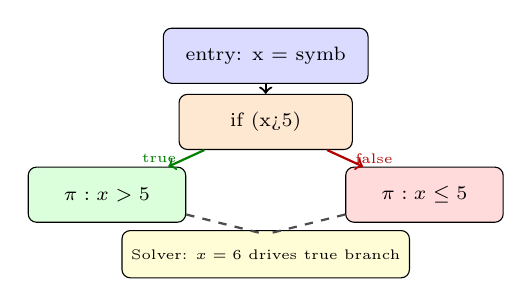
\begin{tikzpicture}[scale=0.84,every node/.style={font=\scriptsize}]
  \node[draw,fill=blue!14,rounded corners=3pt,minimum width=2.6cm,minimum height=0.7cm,align=center] (entry) at (0,2.4) {entry: x = symb};
  \node[draw,fill=orange!18,rounded corners=3pt,minimum width=2.2cm,minimum height=0.7cm,align=center] (br) at (0,1.4) {if (x>5)};
  \node[draw,fill=green!14,rounded corners=3pt,minimum width=2.0cm,minimum height=0.7cm,align=center] (t) at (-2.4,0.3) {$\pi: x>5$};
  \node[draw,fill=red!14,rounded corners=3pt,minimum width=2.0cm,minimum height=0.7cm,align=center] (f) at (2.4,0.3) {$\pi: x\le5$};
  \node[draw,fill=yellow!16,rounded corners=3pt,minimum width=3.0cm,minimum height=0.6cm,align=center,font=\tiny] at (0,-0.6) {Solver: $x=6$ drives true branch};
  \draw[->,thick] (entry) -- (br);
  \draw[->,thick,green!50!black] (br) -- (t) node[midway,left,font=\tiny] {true};
  \draw[->,thick,red!70!black] (br) -- (f) node[midway,right,font=\tiny] {false};
  \draw[dashed,thick,gray!60!black] (t) -- (0,-0.3); \draw[dashed,thick,gray!60!black] (f) -- (0,-0.3);
\end{tikzpicture}
\caption{Symbolic fork. The path constraint accumulates branch conditions; a solver produces concrete inputs for each feasible path, even those guarded by narrow equalities.}
\label{fig:symbolic-fork}
\end{figure}

Path explosion limits pure symbolic execution; \emph{concolic} (concrete+symbolic, e.g., KLEE, SAGE) runs concretely on a seed and uses symbolic reasoning only to flip one branch at a time, marrying fuzzing's scalability with solving's precision. Modern hybrids (AFL+SymCC, Driller) interleave both.

Coverage and corpus quality are observable: track edges covered, corpus size, and executions/sec. A plateau in edges after hours suggests the harness is stuck on a checksum or magic constant; add a dictionary entry or split the harness to isolate the parser from the processor. Seeds from production traffic or unit tests outperform empty seeds by orders of magnitude.

Trade-offs: fuzzing is fast and shallow; symbolic is slow and deep; sanitizers are the oracle both need; coverage is the guide for one and the goal for the other.

\begin{lstlisting}[language=Python]
# Concolic intuition: flip a branch with a solver (pseudocode)
# Path: if x*x == 42: bug()
# Fuzzer may never hit 42; solver solves x*x==42 -> x is not int => unsat, so know branch is dead
import z3
x = z3.Int('x')
s = z3.Solver(); s.add(x*x == 42)
print(s.check())  # unsat -- so the bug branch is unreachable for integers
\end{lstlisting}

% ============================================================
\section{Grammar and Structure-Aware Fuzzing}
\label{sec:grammar-fuzz}
Raw byte mutation fails on highly structured inputs (images, JS, SQL). Grammar-aware fuzzing mutates at the syntax-tree level, preserving validity while exploring semantic branches. Protocol buffers, libprotobuf-mutator and Domato generate inputs that pass the parser but exercise the logic behind it, where the interesting bugs live.

% ============================================================
\section{Triage and Continuous Fuzzing}
\label{sec:triage}
{\sloppy
A crash is not a bug report until it is deduplicated, minimised and root-caused. Cluster by (top N frames of) sanitizer trace, minimise to the shortest reproducer, then bisect to the commit. Patch with a minimal fix that preserves the parser's intent, add the reproducer to the regression corpus under \texttt{corpus/}, and keep fuzzing in CI (OSS-Fuzz model) so the bug class does not return. Gate merges on ``no new sanitizer crash in 5 minutes of fuzzing''; nightly jobs run longer. A bug found in 10 minutes of fuzzing would have been a 10-month incident in production. Track corpus coverage over time; a flat line means the harness is stuck and needs a new dictionary or entry point.
\par}

% ============================================================
\section{From Crash to Fix: A Triage Playbook}
\label{sec:fix-playbook}
{\sloppy
A fuzzer crash is not a CVE until triaged. Steps: (1)~deduplicate by sanitizer trace hash (e.g., \texttt{ASAN\_OPTIONS=}\texttt{dedup\_token}), (2)~minimise with \texttt{afl-tmin} or \texttt{creduce} to the shortest reproducer, (3)~reproduce on a non-instrumented build to rule out sanitizer-only artefacts, (4)~bisect to the commit with \texttt{git bisect}, (5)~patch, (6)~re-fuzz the patched corpus to confirm zero crashes, (7)~add the minimised reproducer to CI as a regression test. Skipping minimisation obscures the root cause; skipping deduplication drowns the team in duplicates.
\par}



\begin{remark}[Fuzzing in CI]
Gate every pull request on 60 seconds of fuzzing with sanitizers on the changed targets; nightly jobs run 8 hours on the full corpus. OSS-Fuzz runs indefinitely on critical open-source projects and has found $>10$k bugs; the cost is a few cores, the benefit is bugs found before adversaries do.
\end{remark}


{\sloppy
\begin{example}[Heartbleed as fuzzing target]
Heartbleed was a missing bounds check: \texttt{memcpy(bp, pl, payload)} where \texttt{payload} was attacker-controlled and larger than \texttt{pl}. A harness that called \texttt{dtls1\_process\_heartbeat} with ASan on random length fields would have crashed instantly. The lesson: even a 10-line harness on the right API would have found a catastrophic bug.
\end{example}
\par}

% ============================================================
\section{Exercises}
\label{sec:ch05-exercises}
{\sloppy
\begin{enumerate}[label=E5.\arabic*, leftmargin=*, itemsep=0.6em]
    \item \textbf{Coverage intuition.} A parser checks \texttt{if (magic==0xDEADBEEF) \{ if (len>100) vuln(); \}}. How many random 32-bit guesses to hit the outer check? Why does coverage guidance help with the inner check but not the outer? How would a dictionary help?
    \item \textbf{Sanitizer choice.} Which sanitizer catches each: (a) heap overflow by 1 byte, (b) use-after-free, (c) read of uninitialised stack variable, (d) signed integer overflow in C, (e) data race? What slowdown/memory cost do you expect for (a)+(b) together?
    \item \textbf{Harness design.} Design a libFuzzer harness for a function \texttt{int decode(const uint8\_t *buf,} \texttt{size\_t len, Image *out)}. What preconditions minimise false positives? How do you avoid state bleed across iterations?
    \item \textbf{Symbolic vs.\ fuzzing.} Give a program where fuzzing needs $>2^{32}$ tries but symbolic solves in one query, and one where symbolic explodes but fuzzing is fast. What hybrid strategy would you use for a real codebase containing both?
    \item \textbf{Crash triage.} You get 1,000 ASan crashes from a fuzz run. Describe the pipeline to deduplicate, minimise, prioritise (exploitable vs.\ benign), and verify a fix, naming the tools and the stopping condition.
\end{enumerate}
\par}

\section*{Chapter Notes}
{\sloppy
AFL by Zalewski; libFuzzer and honggfuzz; coverage-guided fuzzing surveyed in Manes et al.~(2021). ASan/MSan/TSan/UBSan by Serebryany et al.\ (Google). Symbolic execution from King (1976); modern KLEE (Cadar et al., OSDI~2008) and SAGE (Godefroid et al.). Hybrid fuzzing in Stephens et al.~(Driller, 2016) and SymCC. Continuous fuzzing at scale is OSS-Fuzz (Serebryany, 2017).
\par}

% End of Chapter 5
